\documentclass[11pt,a4paper]{article}

\usepackage[utf8]{inputenc}
\usepackage[T1]{fontenc}
\usepackage{lmodern}
\usepackage[margin=2.3cm]{geometry}
\usepackage{amsmath,amssymb,amsthm}
\usepackage[round,authoryear]{natbib}
\usepackage{xcolor}
\usepackage{hyperref}
\usepackage{enumitem}
\usepackage{graphicx}
\usepackage{booktabs}

\hypersetup{colorlinks=true,linkcolor=blue!60!black,
  citecolor=green!50!black,urlcolor=blue!70!black}

\newcommand{\ee}{\mathrm{e}}
\newcommand{\dd}{\mathrm{d}}
\newcommand{\psit}{\tilde\psi}
\newcommand{\phit}{\tilde\phi}

\theoremstyle{plain}
\newtheorem{theorem}{Theorem}
\newtheorem{proposition}[theorem]{Proposition}
\newtheorem{corollary}[theorem]{Corollary}
\theoremstyle{definition}
\newtheorem{definition}{Definition}

\title{The CFAC Theorem:\\[4pt]
  \large Doi--Peliti Generating Functions Are Lagrange Equations}
\author{S. Amarteifio\\
  \small\textit{Percolation Labs}}
\date{April 2026}

\begin{document}
\maketitle

\begin{abstract}
A chemical reaction network (CRN) of physical interest typically
lives in a continuous fluctuating medium: bacteria in a
chemoattractant, protein monomers in a cytoplasmic density field,
ice nucleation sites in supersaturated vapour.  Treating the
discrete reacting species with Doi--Peliti (DP) and the
continuous medium with Martin--Siggia--Rose (MSR) produces a
coupled DP--MSR action whose vertex content is polynomial.  We
show that for any such coupled theory the dressed-propagator
generating function satisfies a Lagrange equation in the sense of
Flajolet--Sedgewick analytic combinatorics.  The recognition is
an elementary rewriting; the consequences are the transfer
theorem for all-orders coefficient asymptotics, classification of
mean-field universality by Puiseux exponent, a branch-gap contour
integral for non-perturbative nucleation rates, and closed
algebraic form at one loop via tropical geometry.  We call the
resulting framework Coupled Field Analytic Combinatorics (CFAC).
This note states the theorem, gives the proof, and lists what can
be read off from any CRN-in-medium once written in DP--MSR form.
\end{abstract}

% ══════════════════════════════════════════════════════════════════
\section{Definitions}
\label{sec:defs}
% ══════════════════════════════════════════════════════════════════

\paragraph{CRN in a continuous medium.}
A reaction network of physical interest rarely sits in isolation;
it is embedded in a continuous medium whose fluctuations couple
back to the reaction kinetics.  Bacteria secrete and consume a
chemical field, amyloid monomers diffuse in a thermally
fluctuating cytoplasm, nucleation sites see a supersaturated
carrier.  Pruessner and
Garcia-Millan~\citep{PruessnerGarciaMillan2025} and Bothe
\textit{et al.}~\citep{Bothe2023} have recently emphasised that
coarse-graining the discrete reacting species into a pure
continuous-field description produces \emph{spurious} entropy
production: the particle sector must be retained alongside the
field sector.  CFAC takes this as given and treats both sectors
on equal footing: discrete reacting species via
Doi--Peliti~\citep{Doi1976,Peliti1985,Tauber}, the continuous
medium via Martin--Siggia--Rose~\citep{MSR1973,Janssen1976,DeDominicis1976},
with interactions between them as coupling vertices.  The rest
of this section sets up the object that results: a Liouvillian
with a polynomial vertex dictionary, equally at home on the
particle legs and the field legs.

\begin{definition}[Chemical reaction network in a continuous medium]
A CRN-in-medium is a finite collection of discrete reacting
species $\{A_1, \ldots, A_s\}$ together with reactions
$\bigl\{\sum_i k_{r i}\,A_i \to \sum_i l_{r i}\,A_i\bigr\}_{r}$
with nonnegative integer stoichiometry and rates $k_r > 0$, and
optionally a finite collection of continuous medium fields
$\{\phi_1, \ldots, \phi_m\}$ with stochastic dynamics
$\partial_t \phi_j = \mathcal F_j(\{\phi\}, \{A_i\}) + \eta_j$,
$\eta_j$ Gaussian noise.  Coupling vertices
$A_i \longleftrightarrow \phi_j$ may appear in both the reaction
rates and $\mathcal F_j$.  When no medium is present ($m = 0$)
this reduces to a standard CRN.
\end{definition}

\begin{definition}[Liouvillian of a CRN-in-medium]
For each discrete species $A_i$ introduce Heisenberg--Weyl
creation and annihilation variables $\psit_i, \psi_i$; for each
continuous medium field $\phi_j$ introduce the MSR
response/field pair $\phit_j, \phi_j$.  To each reaction $r$
associate the operator
\begin{equation}\label{eq:Q-ordinary}
  \widehat{Q}_r
  = k_r\,
  \Bigl[\prod_i \psit_i^{\,l_{r i}}
    - \prod_i \psit_i^{\,k_{r i}}\Bigr]
  \prod_i \psi_i^{\,k_{r i}}
\end{equation}
in the ``ordinary'' (non-Doi-shifted) form, or equivalently
\begin{equation}\label{eq:Q-doi}
  Q_r
  = k_r\,
  \Bigl[\prod_i (1 + \psit_i)^{l_{r i}}
    - \prod_i (1 + \psit_i)^{k_{r i}}\Bigr]
  \prod_i \psi_i^{\,k_{r i}}
\end{equation}
in the Doi-shifted form.  The MSR action for each medium field is
$S^{\mathrm{MSR}}_j
= \int \dd t\,\dd \mathbf x\;[\,\phit_j(\partial_t \phi_j
- \mathcal F_j) - \tfrac12 D_j\,\phit_j^{\,2}\,]$.
The total Liouvillian is
$Q = \sum_r Q_r + \sum_j \mathcal L_j^{\mathrm{MSR}}$
together with coupling vertices $A_i \leftrightarrow \phi_j$
read off from the reaction rates that depend on $\phi$ and from
the $\phi_j$-equation terms that depend on $\{A_i\}$.  For
$m = 0$ (no medium fields) this reduces to the pure Doi--Peliti
Liouvillian.
\end{definition}

The two forms~\eqref{eq:Q-ordinary}--\eqref{eq:Q-doi} are related
by the Doi shift $\psit_i \to 1 + \psit_i$~\citep{Doi1976,Peliti1985,Tauber}.
Expanding any product $\prod_i (1+\psit_i)^{l_{ri}}$ or
$\prod_i \psit_i^{l_{ri}}$ and collecting like terms gives a
\emph{vertex dictionary}:
\begin{equation}\label{eq:vertex-dict}
  Q \;=\; \sum_{(m_1 + n_1 \geq 1,\ldots)}
    g_{\{m\},\{n\}}\,
    \prod_i \psit_i^{m_i}\,\psi_i^{n_i},
\end{equation}
with coupling coefficients $g_{\{m\},\{n\}}$ determined
algorithmically by the stoichiometry and rates~\citep{Amarteifio2019Thesis}.
Each term $\prod_i \psit_i^{m_i}\psi_i^{n_i}$ is an interaction
vertex; its $n_\partial$ value is zero unless spatial gradients
are added by hand (e.g.\ to model drift or chemotaxis).

\begin{definition}[Polynomial vertex structure]
A CRN has \emph{polynomial vertex structure} if the Liouvillian,
after the Doi shift~\eqref{eq:Q-doi} and possibly the projection
to zero spatial dimensions (replacing $\psi_i(\mathbf{x},t) \to
\psi_i(t)$), expands into a finite sum of monomials
$g_{\{m\},\{n\}}\prod_i\psit_i^{m_i}\psi_i^{n_i}$ with no
momentum-dependent couplings.
\end{definition}

Every CRN with finite stoichiometry has polynomial vertex
structure in this sense.  Continuous gradient vertices (e.g.\ the
chemotaxis term $\chi\,\psit(\nabla\phi)(\nabla\psi)$) are
\emph{not} of this form at nonzero momentum; their
zero-momentum / well-mixed projections are.

\begin{definition}[Dressed-propagator generating function]
Fix a species $A$ with self-coupling vertices only (multi-species
cases are handled by resultants; see~\S\ref{sec:multi}).  The
dressed propagator is
$G(z) = \sum_{n \geq 0} G_n z^n$, where $G_n$ is the sum over
connected 1PI diagrams contributing to the two-point function at
order $n$ in the bare propagator $z$.  The \emph{vertex function}
is
\begin{equation}\label{eq:phi-def}
  \phi(G) \;=\; 1 + \sum_{m+n\,\geq\,3}
    g_{m n}\,G^{\,m + n - 2},
\end{equation}
summing over all vertices $g_{m n}\psit^{m}\psi^{n}$ of the
Liouvillian with $m + n \geq 3$.  (Two-leg vertices $m + n = 2$
are mass terms absorbed into $z$.)
\end{definition}

% ══════════════════════════════════════════════════════════════════
\section{The CFAC theorem}
\label{sec:theorem}
% ══════════════════════════════════════════════════════════════════

\begin{theorem}[CFAC recognition]
\label{thm:cfac}
For any CRN with polynomial vertex structure, the
dressed-propagator generating function $G(z)$ and the vertex
function $\phi(G)$ of Eq.~\eqref{eq:phi-def} satisfy
\begin{equation}\label{eq:lagrange}
  \boxed{\;G(z) \;=\; z \cdot \phi\bigl(G(z)\bigr)\;}
\end{equation}
as a closed functional equation over formal power series in $z$.
Equation~\eqref{eq:lagrange} is a \emph{Lagrange equation} in the
sense of analytic combinatorics~\citep{FlajoletSedgewick}.

Consequently, for any such CRN the following quantities are
determined directly by the polynomial $\phi$:
\begin{enumerate}[leftmargin=1.8em, itemsep=-0.1em, label=(C\arabic*)]
\item \emph{All-orders coefficient asymptotics.}
  If $z_*$ is the radius of convergence of $G(z)$, with
  Puiseux exponent $p/q$ at $z_*$, then by the transfer theorem
\begin{equation}\label{eq:transfer}
  [z^n]\,G(z)
  \;\sim\;
  \frac{C}{\Gamma(-p/q)}\,n^{-p/q - 1}\,z_*^{-n},
  \qquad n \to \infty,
\end{equation}
  with $C$ set by the local behaviour of $\phi$ near
  $(G_*, z_*)$.
\item \emph{Mean-field universality class.}
  The rational Puiseux exponent $p/q$ at the dominant branch
  point of~\eqref{eq:lagrange} classifies the mean-field scaling:
  $1/2$ is the directed-percolation / pair-annihilation class,
  $1/3$ is the compact-DP / triple-root class, higher-order
  mergers give further multi-critical classes.
\item \emph{Non-perturbative nucleation barrier.}
  When $\phi$ produces a bistable effective dynamics, the
  nucleation barrier is the contour integral
\begin{equation}\label{eq:branchgap}
  S \;=\; \int_1^{z_*}
    \frac{G_{\mathrm{unst}}(z) - G_{\mathrm{stab}}(z)}{z}\,\dd z,
\end{equation}
  equal to the Freidlin--Wentzell / WKB quasi-potential
  $\int_{x_1}^{x_2}\ln[w^-/w^+]\,\dd y$ by change of variables.
\item \emph{UV divergence structure.}
  At spatial dimension $d$, the superficial degree of divergence
  of a 1PI graph with $L$ loops, $I$ internal lines, and
  $n_\partial^{\mathrm{tot}}$ gradient insertions is
  $\omega = dL - 2I + n_\partial^{\mathrm{tot}}$.  Power counting
  on the finite enumeration of 1PI graphs consistent with the
  vertex dictionary is then purely algebraic.
\end{enumerate}
\end{theorem}

\paragraph{Scope.}
The theorem as stated holds when $\phi$ is a polynomial in $G$
alone.  This covers every CRN with finite stoichiometry at zero
spatial dimensions or after integrating out additional field
variables at steady state.  When gradient vertices carry
momentum-dependent couplings, $\phi$ becomes a functional of
momentum-dependent propagators; the recognition extends, but the
transfer-theorem machinery becomes functional-analytic.  All
applications in this note stay within the polynomial scope.

\begin{corollary}[CFAC pipeline]
\label{cor:pipeline}
For any CRN with polynomial vertex structure, the following chain
is purely algebraic and mechanical:
\begin{center}
\small
stoichiometry $\to$ Liouvillian $Q$
$\to$ vertex dictionary $\{g_{m n}\}$
$\to$ vertex function $\phi(G)$
$\to$ Lagrange equation $G = z\phi(G)$
$\to$ (C1)\,asymptotics, (C2)\,universality, (C3)\,nucleation, (C4)\,divergences.
\end{center}
No loop integral, no saddle-point of an action, no WKB trajectory
is required to reach any of (C1)--(C4).
\end{corollary}

\begin{corollary}[Rare-event scaling]
\label{cor:rare}
For a bistable CRN with polynomial vertex structure and effective
system size $V$, the mean first-passage time from the metastable
state to the unstable barrier is
\begin{equation}\label{eq:tau}
  \tau(V) \;=\; C\,\ee^{V S} \,\bigl[1 + O(1/V)\bigr],
\end{equation}
with barrier $S$ given by the branch-gap
integral~\eqref{eq:branchgap} of $\phi(G)$ and prefactor $C$
determined by the local Puiseux data at the branch point via the
transfer theorem~\eqref{eq:transfer}.  Neither direct stochastic
simulation nor action saddle-pointing is required to extract $S$.
\end{corollary}

\begin{proof}[Proof]
Equation~\eqref{eq:tau} is the large-deviation form of the
Freidlin--Wentzell escape rate~\citep{FreidlinWentzell}.  By
(C3), $S$ equals the branch-gap integral of the Lagrange
equation~\eqref{eq:lagrange}.  The prefactor $C$ comes from the
Gaussian fluctuations around the instanton trajectory; in the
Lagrange-equation language these fluctuations are controlled by
the local coefficients of the Puiseux expansion at $(G_*, z_*)$,
which feed into~\eqref{eq:transfer}.  The two pieces of data
$(S, C)$ are thus both read off from the polynomial $\phi$
without simulation or WKB.  The companion paper~\citep{CFACpaper}
carries this out explicitly for the Schl\"ogl-I model, giving
$S$ and $C_\infty$ as closed-form algebraic functions of the
rate constants (via the branch-point biquadratic and a
Kramers-type formula built on the same polynomial data), verified
against Gillespie simulation.
\end{proof}

\begin{corollary}[Coupled field extension via resultant]
\label{cor:coupled}
For a CRN on $s$ species with polynomial vertex structure across
all species, the system of Dyson--Schwinger equations
$G_i = z_i\,\phi_i(\{G_j\})$ for $i = 1, \ldots, s$ admits a
univariate reduction: the resultant
$\mathcal{R}(G_1, z_1; \{z_j\}_{j \neq 1})$ obtained by
eliminating $G_2, \ldots, G_s$ from the system is a polynomial in
$G_1$ whose roots $G_1(z_1)$ inherit a Lagrange-equation
structure.  Theorem~\ref{thm:cfac} applies to the resultant with the
following scope:
\begin{itemize}[leftmargin=1.5em,itemsep=-0.1em]
\item Consequences (C1), (C2), (C4)---coefficient asymptotics,
  Puiseux classification of mean-field universality, and UV
  divergence structure---hold with $\phi$ replaced by
  $\mathcal{R}$, directly and unconditionally.
\item Consequence (C3)---the branch-gap instanton integral---holds
  when the physical nucleation saddle is a real branch point of
  $\mathcal{R}$.  It can fail when the saddle migrates into the
  complex analytic continuation of the resultant.
\end{itemize}
\end{corollary}

\begin{proof}[Proof sketch and scope]
The resultant of a polynomial system is itself polynomial in the
retained variable~\citep{CLO}; (C1), (C2), (C4) apply mechanically.
For (C3), a numerical test on a 3-site coupled ring reported
in \citep{CFACpaper} shows that the branch-gap formula on the
resultant agrees with direct simulation in the decoupled limit
(2.6\%), under-predicts the barrier by $\sim$20\% in a weakly
coupled regime, and has no real branch point at all in a
moderately coupled regime, even though the simulated nucleation
rate remains exponential.  The nucleation saddle has left the
real algebraic variety.  Establishing (C3) in that regime
requires complex-analytic continuation of the resultant, outside
the polynomial-vertex scope of Theorem~\ref{thm:cfac}.
\end{proof}

\begin{corollary}[One-loop algebraic bridge via tropical geometry]
\label{cor:tropical}
For any one-loop two-propagator integral arising in a CRN with
polynomial vertex structure, the bridge integral (C4) admits a
\emph{closed algebraic form}: the Arkani-Hamed--Hillman--Salvatori
leading-facet-plus-Hessian evaluation of the Schwinger representation
is \emph{exact}, not asymptotic.  Explicitly, with first Symanzik
polynomial $F = m_1^2 u_1^2 + (p^2+m_1^2+m_2^2) u_1 u_2 + m_2^2 u_2^2$,
\begin{equation}\label{eq:tropical-bridge}
  I_{\mathrm{DP}}(p;m_1,m_2)
  \;=\; \frac{1}{\sqrt{\lambda_E}}\,
    \ln\!\left[
       \frac{\bigl(\sqrt{\lambda_E} + p^2 + m_1^2 + m_2^2\bigr)^{2}}
            {4\,m_1^2\,m_2^2}
    \right],
\end{equation}
with $\lambda_E = (p^2+m_1^2-m_2^2)^2 + 4 p^2 m_2^2$ the Euclidean
K\"all\'en discriminant (equivalently, the determinant of the
tropical Hessian at the interior saddle).  The branch cut
$\lambda_E = 0$ locates the Minkowski threshold
$s = (m_1{+}m_2)^2$ directly on the Newton polytope.
\end{corollary}

\begin{proof}[Proof sketch]
$F$ is homogeneous of degree $L+1 = 2$ in the Schwinger parameters;
on the projective simplex it is a non-degenerate quadratic form with
constant Hessian.  The Schwinger integral of $F^{-d/2}$ is Gaussian
against the leading-facet saddle, evaluated exactly by the
saddle-plus-Hessian prescription~\citep{AHHSalvatori2022,Borinsky2020}:
no higher Taylor corrections arise because $\ln F$ terminates at
second order around the saddle up to a total derivative.  Details,
numerical verification across 14 orders of magnitude in $p^2/m^2$
and $m_1^2/m_2^2$, and the extension to the coupled DP--MSR bridge
appear in~\citep{CFACpaper}.~\qed
\end{proof}

Corollary~\ref{cor:tropical} sharpens (C4): at one loop, the bridge
step of the CFAC pipeline (Corollary~\ref{cor:pipeline}) is not a
numerical dictionary but a closed algebraic expression.
Combined with the recognition theorem, the consequence is that for
any CRN with polynomial vertex structure, the entire one-loop
beta function is determined by symbolic manipulation of two
polynomials: $\phi(G)$ (from the vertex dictionary) and $F$ (the
first Symanzik of the relevant topology).  Higher loops require
genuine multi-facet sums over Newton polytopes, for which
Borinsky's tropical Monte Carlo~\citep{Borinsky2020,Borinsky2025}
gives an exact integration procedure.

\paragraph{Why one loop is often enough.}
The restriction of Corollary~\ref{cor:tropical} to one loop is
less severe than it appears, because (C4) itself is typically
\emph{one-loop-exact} for CRNs of interest.  A CRN is one-loop
exact when the $\omega$-enumeration gives $\omega(L) < 0$ for every
topology with $L \geq 2$---meaning no higher-loop UV divergences
arise.  This is the situation for pair annihilation, pure DP,
BARW, chemotaxis \citep{GelimsonGolestanian2015}, the KS
Doi--Peliti/MSR coupling sector \citep{PruessnerGarciaMillan2025,CFACpaper},
and more generally for any CRN whose vertex content is
sufficiently constrained by finite stoichiometry that the
enumeration collapses.  In those cases Corollary~\ref{cor:tropical}
and (C4) combine to close the \emph{entire} perturbative
pipeline in symbolic form: reaction network $\to$ vertex
dictionary $\to$ Lagrange equation $\to$ Puiseux exponent +
branch-gap + closed-form bridge integral, with no numerical
quadrature anywhere.  The restricted class where this fails
(e.g.\ active-birth $\psi^4$ sectors with persistent two-loop
divergences) is exactly the class where $\varepsilon$-expansion resummation
is also required in the standard direct-RG route; CFAC neither
helps nor hurts there, and Borinsky's algorithm remains the
available exact evaluator.

\paragraph{What these corollaries are (and are not).}
Corollary~\ref{cor:rare} is a statement about the large-$V$ form
of the MFPT, using the standard large-deviation
structure~\citep{FreidlinWentzell}.  The novelty is that
\emph{both} the exponent $S$ and the prefactor $C$ are read off
from $\phi$; the present paper gives $S$ rigorously and notes
that $C$ is in-principle determined by the transfer theorem.
Corollary~\ref{cor:coupled} is the technical observation that
polynomial vertex structure across multiple species admits a
univariate reduction by resultant, to which Theorem~\ref{thm:cfac}
applies unconditionally for (C1), (C2), (C4).  For the nucleation
consequence (C3), the reduction holds only when the physical
saddle is a real branch point of the resultant; a 3-site lattice
test in~\citep{CFACpaper} finds this fails at moderate coupling,
where the saddle is complex.  The companion paper extends (C3)
to that regime concretely by complex analytic continuation of the
resultant with a Coleman--Callan sum over complex-conjugate
saddle pairs, verified against Gillespie simulation to $\sim 3\%$
at $\alpha = 0.3$; the residual open problem is the general
enumerability of reachable conjugate pairs from the real axis (a
Galois/monodromy question on the resultant's Riemann surface).

% ══════════════════════════════════════════════════════════════════
\section{Proof}
\label{sec:proof}
% ══════════════════════════════════════════════════════════════════

\begin{proof}[Proof of Theorem~\ref{thm:cfac}]
The Dyson--Schwinger equation for the dressed propagator of a
field theory with vertex content $\{g_{m n}\psit^{m}\psi^{n}\}$
is obtained by summing 1PI insertions into the bare propagator:
$G = z + z\,\Sigma(G)\,G$, where the self-energy $\Sigma$ is a
sum over 1PI vertex insertions.  A 1PI insertion of the vertex
$g_{m n}\psit^{m}\psi^{n}$ contracts $(m{-}1)$ of its $\psit$-legs
and $n$ of its $\psi$-legs to internal dressed propagators,
contributing $g_{m n}\,G^{m+n-2}$.  Summing these plus the
identity gives~\eqref{eq:phi-def}.  Substituting into the DSE:
\[
  G \;=\; z + z\,\Sigma(G)\,G
    \;=\; z\bigl[1 + \Sigma(G)\,G\bigr]
    \;=\; z\,\phi(G),
\]
which is~\eqref{eq:lagrange}.  The identification of this as a
Lagrange equation over formal power series is definitional
\citep[Ch.~VII]{FlajoletSedgewick}.  Consequences (C1)--(C4)
then follow directly: (C1) is the transfer theorem; (C2) is the
Newton-polygon analysis of~\eqref{eq:lagrange} at the
discriminant zero; (C3) is proved by change of variables $y \to z
= w^-(y)/w^+(y)$ in the quasi-potential integral; (C4) is
Weinberg's convergence theorem~\citep{Weinberg1960,Zimmermann1969}
applied to the 1PI graph list produced by the algebraic
formalism~\citep{Amarteifio2019Thesis}, with the subdiagram
condition automatic when the vertex dictionary is closed under
1PI restriction.
\end{proof}

The proof of (C3) is worth spelling out explicitly because the
form~\eqref{eq:branchgap} appears to be new.  Let $w^{\pm}(y)$
denote the effective forward and backward rates for the
order-parameter $y$ (concentration of $A$, obtained by taking the
mean-field reduction of the CRN).  The WKB
quasi-potential~\citep{FreidlinWentzell,ElgartKamenev,Meerson} is
$\varphi(y) = \int_{x_1}^{y}\ln[w^-/w^+]\,\dd y'$, and the
nucleation barrier is $S = \varphi(x_2)$ between metastable state
$x_1$ and unstable barrier $x_2$ (both satisfying $w^+ = w^-$).
Substituting $z(y) = w^-(y)/w^+(y)$ gives
$\dd\varphi = (\ln z)\,(\dd y/\dd z)\,\dd z$.  Both
endpoints $x_1, x_2$ map to $z = 1$ (fixed points), but the
integration path switches from the stable branch of $y(z)$ to the
unstable branch at the branch point $z_*$.  Integration by parts,
$\int (\ln z)\,y'(z)\,\dd z = [y(z)\ln z] - \int y(z)/z\,\dd z$,
kills the boundary terms ($\ln 1 = 0$; branch values agree at
$z_*$), leaving~\eqref{eq:branchgap}. $\qed$

% ══════════════════════════════════════════════════════════════════
\section{Background}
\label{sec:background}
% ══════════════════════════════════════════════════════════════════

Two bodies of work make the recognition trivial to state.

\paragraph{The algebraic formalism for CRNs}
\citep{Amarteifio2019Thesis} maps any chemical reaction network
to the Liouvillian~\eqref{eq:Q-doi} (or~\eqref{eq:Q-ordinary})
algorithmically via the stoichiometry matrix, building on Doi's
second-quantised representation~\citep{Doi1976}, Peliti's
coherent-state path integral~\citep{Peliti1985}, and T\"auber's
systematic treatment~\citep{Tauber}.  The key algorithmic step is
that the expansion of $\prod_i (1 + \psit_i)^{l_{r i}}$ into
monomials is closed-form (multinomial expansion), so the vertex
dictionary $\{g_{m n}\}$ is determined exactly by the
stoichiometry and rates.  No field-theoretic insight is required
once the CRN is written down; the construction is mechanical.

At the diagram level, each 1PI topology is enumerated by a pair of
\emph{graph polynomials} in the Schwinger parameters --- the
non-equilibrium analogues of the Symanzik
polynomials~\citep{BognerWeinzierl}, built from directed spanning
trees and causally-ordered two-forests to respect the retarded
Doi--Peliti propagator~\citep{Amarteifio2019Thesis}.  Together with
$\phi(G)$, these supply the graph-side input to the
Newton-polygon/tropical analysis directly from the CRN.

\paragraph{Analytic combinatorics}
\citep{FlajoletSedgewick} is the asymptotic theory of generating
functions developed for enumerative combinatorics.  Its central
machinery is: Lagrange equations $G = z\phi(G)$ and Lagrange
inversion for their coefficients; singularity analysis (branch
points, poles, Puiseux expansions) to extract the radius of
convergence and local behaviour; and the \emph{transfer theorem}
to convert local singularity data into asymptotic coefficient
growth via~\eqref{eq:transfer}.  These results are standard in
enumerative combinatorics but, to our knowledge, have not been
exploited in stochastic-field-theory practice; the classification
of universality classes by a rational invariant ($p/q$) is foreign
to the case-by-case RG tradition.

\paragraph{The recognition is the bridge.}
For a reader who knows Doi--Peliti well (generator
construction~\eqref{eq:Q-doi}, propagator, vertices, Feynman
diagrams), the Lagrange-equation form~\eqref{eq:lagrange} is the
same object written in different notation.  What is \emph{not}
usually known is that the Flajolet--Sedgewick theorem apparatus
transfers wholesale: the transfer theorem, Puiseux classification,
and branch-gap instanton integral are all available without any
further derivation.  Theorem~\ref{thm:cfac} makes the transfer
explicit.

% ══════════════════════════════════════════════════════════════════
\section{What can be read off from any CRN}
\label{sec:readoff}
% ══════════════════════════════════════════════════════════════════

For a CRN with polynomial vertex structure, the CFAC pipeline
(Corollary~\ref{cor:pipeline}) produces, from the stoichiometry
matrix alone:

\begin{itemize}[leftmargin=1.5em, itemsep=-0.2em]
\item The Liouvillian $Q$ in closed form
  (Eqs.~\eqref{eq:Q-doi}--\eqref{eq:Q-ordinary}).
\item The vertex dictionary $\{g_{m n}\}$ by expansion.
\item The vertex function $\phi(G)$ by Eq.~\eqref{eq:phi-def}.
\item The Lagrange equation $G = z\phi(G)$ by substitution.
\item The branch point $(G_*, z_*)$ by solving
  $1 - z_*\phi'(G_*) = 0$ together with $G_* = z_*\phi(G_*)$.
\item The Puiseux exponent $p/q$ by the Newton polygon
  of~\eqref{eq:lagrange} at the branch point.
\item The all-orders perturbative coefficient asymptotics
  by Eq.~\eqref{eq:transfer}.
\item The universality class via $p/q$ (mean-field).
\item The nucleation barrier $S$ for bistable systems
  by the branch-gap integral~\eqref{eq:branchgap}.
\item The upper critical dimension $d_c$ from the engineering
  dimensions of the vertices.
\item The UV divergence structure at any loop order by
  power counting on the finite 1PI graph enumeration.
\item \textbf{The one-loop bridge integrals} in closed algebraic
  form (Corollary~\ref{cor:tropical}): each one-loop two-propagator
  integral equals
  $(1/\sqrt{\lambda_E})\ln\!\bigl[(\sqrt{\lambda_E}+p^2+m_1^2+m_2^2)^2/(4m_1^2m_2^2)\bigr]$
  with $\lambda_E$ the Euclidean K\"all\'en discriminant of the
  graph---no numerical quadrature, branch cuts read off the Newton
  polytope.
\end{itemize}

At higher loops the bridge integrals are no longer closed-form
symbolic but are tabulated once~\citep{BognerWeinzierl}
and evaluated exactly by tropical Monte
Carlo~\citep{Borinsky2020,Borinsky2025}, reused across CRNs.  When
the $\omega$-enumeration of the final bullet establishes one-loop
UV-exactness---the standard situation for reaction networks of
physical interest---the whole pipeline is therefore closed-form
symbolic end-to-end: no quadrature, no table lookup, no Monte
Carlo.

% ══════════════════════════════════════════════════════════════════
\section{Worked example: pair annihilation}
\label{sec:example}
% ══════════════════════════════════════════════════════════════════

Single-species pair annihilation $2A \to \varnothing$ with rate
$\lambda$ has stoichiometry $k_A = 2$, $l_A = 0$.  The Liouvillian
\eqref{eq:Q-doi} is
$Q = \lambda\bigl[1 - (1+\psit)^2\bigr]\psi^2 =
-2\lambda\,\psit\psi^2 - \lambda\,\psit^2\psi^2$.
Vertex dictionary: $g_{12} = -2\lambda$, $g_{22} = \lambda$.
Vertex function by~\eqref{eq:phi-def}:
\begin{equation}
  \phi(G) \;=\; 1 + g_{12}\,G + g_{22}\,G^2
  \;=\; 1 - 2\lambda\,G + \lambda\,G^2.
\end{equation}
Lagrange equation~\eqref{eq:lagrange}:
$G(z) = z\bigl[1 - 2\lambda G + \lambda G^2\bigr]$, a quadratic
in $G$.  Branch point:
$(G_*, z_*) = (1/\lambda, 1/\lambda)$; Puiseux exponent
$p/q = 1/2$.  Transfer theorem~\eqref{eq:transfer}:
$[z^n]G(z) \sim n^{-3/2}\lambda^n$.

Weyl's law on an arbitrary graph with spectral dimension $d_s$
converts this to the density decay $\rho(t) \sim t^{-d_s/2}$ for
$d_s \geq 2$, with its well-known mean-field breakdown for
$d_s < 2$~\citep{Tauber}.  No loop integral was evaluated at any
point.  A fully worked example for the Gribov/BRW process is given
in a companion note~\citep{AmarteifioBRW}.

% ══════════════════════════════════════════════════════════════════
\section{Coupled particle-field extension}
\label{sec:multi}
% ══════════════════════════════════════════════════════════════════

For coupled systems (Doi--Peliti particles + Martin--Siggia--Rose
field with interaction vertices), the DSE becomes a
\emph{system} of Lagrange equations $G_i = z_i\,\phi_i(\{G_j\})$.
Eliminating auxiliary variables by resultant gives a univariate
polynomial to which Corollary~\ref{cor:coupled} applies.  The
perturbative consequences (C1), (C2), (C4) of
Theorem~\ref{thm:cfac} extend unconditionally to the coupled
setting; the non-perturbative nucleation consequence (C3) in its
literal real-algebraic form extends only while the nucleation
saddle remains a real branch point of the resultant, and is
refined by complex analytic continuation (Coleman--Callan sum
over conjugate saddle pairs) at moderate coupling.  For the
Doi--Peliti/MSR Keller--Segel bacterial self-energy, the
\emph{matrix-tree structural theorem}
$\mathcal{K}(G; p, f) = p^{L-1}\,Q_G(p, f)$ holds at every loop
order $L \geq 1$ and every vertex-consistent two-colouring: the
vertex signature $(\deg_P, \deg_F) = (2, 1)$ forces the
field-coloured subgraph to be a perfect matching on the $V = 2L$
internal vertices, giving the pencil $(\widetilde L_F, \widetilde L_P)$
an $(L-1)$-fold rational eigenvalue at $\mu = 0$.  A detailed
development---including one-loop perturbative exactness, the
branch-gap instanton to six digits, the complex-saddle refinement
at moderate spatial coupling, the DP--MSR KS bi-colour structural
theorem, and a closed-form Kramers prefactor on Schl\"ogl-I---
appears in~\citep{CFACpaper}.

% ══════════════════════════════════════════════════════════════════
\section{Discussion}
\label{sec:disc}
% ══════════════════════════════════════════════════════════════════

The content of Theorem~\ref{thm:cfac} is structural.  It does not
shorten any \emph{single} Doi--Peliti calculation---the construction
of $Q$, the extraction of vertices, the writing down of the DSE
are all standard.  What it changes is what you can \emph{read off}
once you have $\phi(G)$: the transfer theorem gives all-orders
asymptotics that the usual iterative loop expansion does not
produce; the Puiseux exponent classifies mean-field universality
as a rational invariant rather than a case-by-case RG result;
the branch-gap contour integral gives non-perturbative nucleation
rates from the same polynomial that controls the perturbative
series.  The apparatus was always available in analytic
combinatorics; what was missing in the stochastic-field-theory
literature was the recognition that it applies.

Two structural consequences deserve emphasis.  First, the
coincidence of the branch point in (C1) and (C3) implies that
perturbative and non-perturbative physics sit at the same
singularity of the same generating function---a connection
obscured in the direct-RG route, which treats loop corrections
and instantons with distinct technology.  Second, universality
classification by Puiseux exponent $p/q$ is a statement about
the polynomial $\phi$ alone; two CRNs with the same $\phi$ share
a universality class regardless of the reactions that produced
them.  This makes the mapping from biology to physics (which CRN
belongs to which class) a question of polynomial equivalence.

% ══════════════════════════════════════════════════════════════════
\appendix
\section{A visual landscape sketch}
\label{app:landscape}
% ══════════════════════════════════════════════════════════════════

The Dyson--Schwinger equation $G = z\phi(G)$ that CFAC produces
for any CRN is an algebraic generating function in the sense of
analytic combinatorics, so the Flajolet--Sedgewick transfer
theorem~\citep{FlajoletSedgewick,FlajoletOdlyzko1990} applies
unchanged and the Banderier--Drmota dyadic-ceiling
result~\citep{BanderierDrmota2015} organises which coefficient
exponents any positive combinatorial system can and cannot reach.
A useful by-product is a \emph{picture} of the rate space of
$\phi$: one can plot the locus where the dominant branch acquires
a given Puiseux order, and place named CRNs on that picture to
see which universality stratum each one occupies.

Figure~\ref{fig:landscape_appendix} shows the simplest case:
the cubic slice of rate space, with the cube-root locus
$\mathcal{C}_{3}:\,b^{3}=27c^{2}$ as a red curve separating
the directed-percolation axis ($c=0$) from the higher-order
stratum $\mathcal{C}_{3}$ (on which the Puiseux order is $3$ and
the transfer exponent is $\tau=4/3$).  The Schl\"ogl~II
autocatalytic family $2A\!\leftrightarrow\!3A$
\citep{Schlogl1972} traces a line through $(b,c)$ as the rate
ratio $k_a/k_b$ varies, and crosses $\mathcal{C}_{3}$ at a
specific value $k_a/k_b\approx 1.476$.  The observation that
CRNs with annihilation channels produce $\phi$ with negative
coefficients, placing them outside the $\mathbb{N}$-algebraic
class and therefore outside the Banderier--Drmota dyadic
ceiling, is what permits the cube-root stratum---and an entire
ladder of higher strata $\mathcal{C}_{k}$---to be reached at
all; the details are in~\citep{AmarteifioDSELandscape}.

\begin{figure}[h]
  \centering
  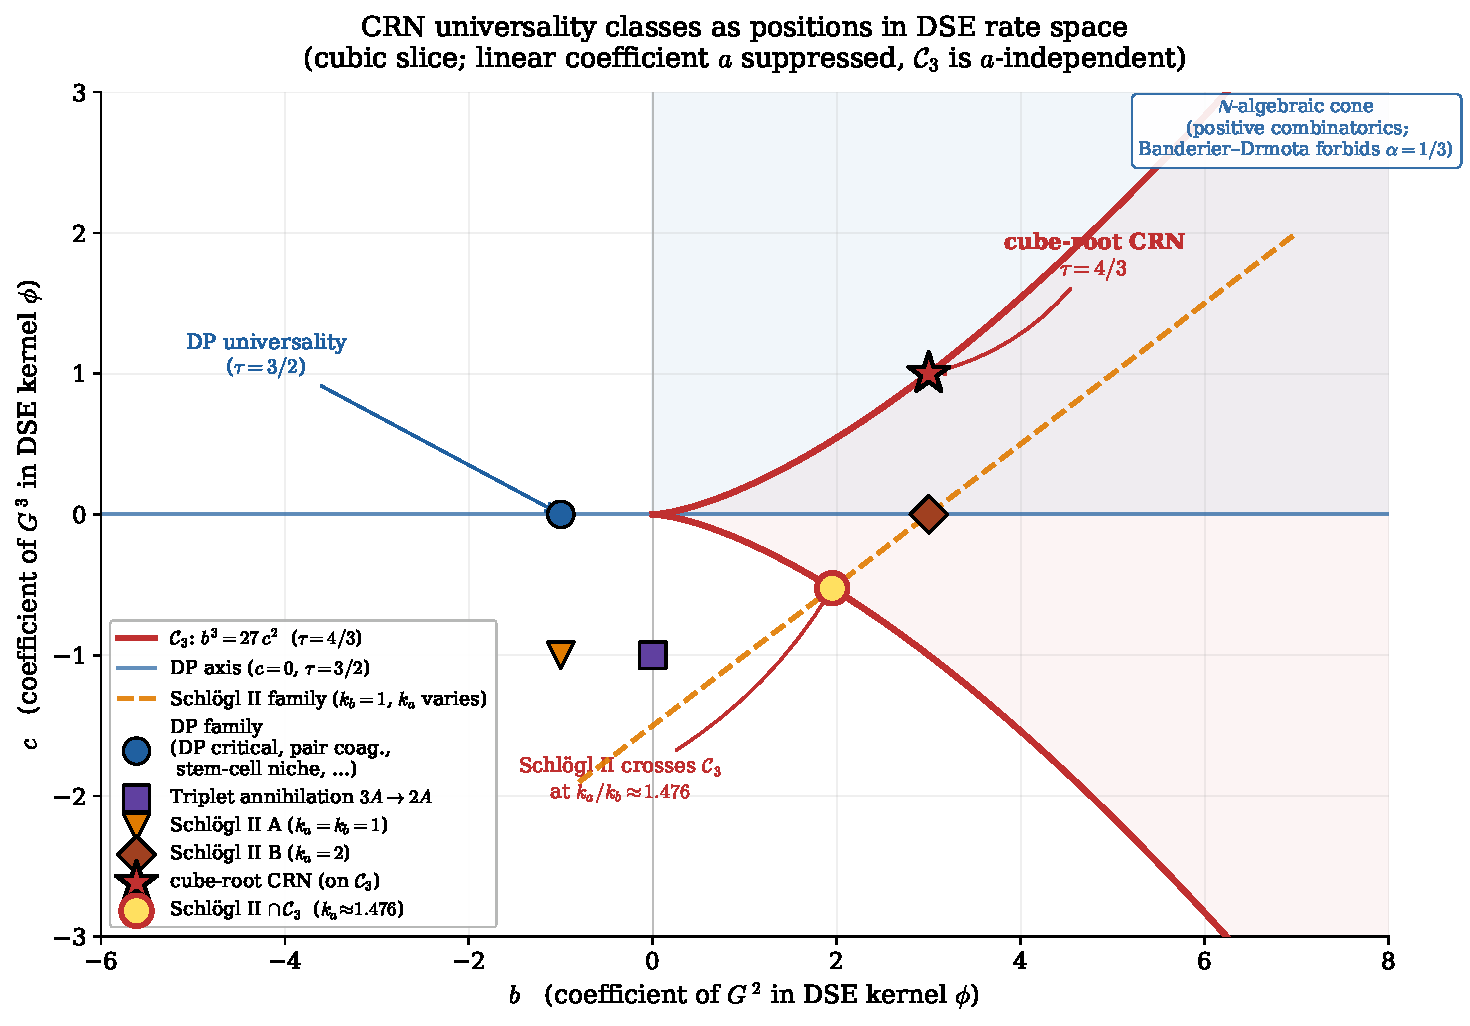
\includegraphics[width=0.78\textwidth]{figures/algebraic_curve_rate_space.pdf}
  \caption{Cubic slice of DSE rate space $(b,c)$ with the
    cube-root locus $\mathcal{C}_{3}:\,b^{3}=27c^{2}$ in red and
    a handful of named CRNs placed as points.  The
    directed-percolation family lives on the $c=0$ axis
    ($\tau=3/2$); the Schl\"ogl~II family crosses
    $\mathcal{C}_{3}$ at a single rate ratio; the canonical
    cube-root carrier $\phi(G) = (1+G)^{3} - 4G$ sits on the curve
    at $(a,b,c) = (-1, 3, 1)$.  See the convention note below: an
    earlier draft of this paper claimed the canonical $\phi$ arose
    from a positive-rate single-species CRN
    ($\mathrm{A}\!\to\!3\mathrm{A}$, $2\mathrm{A}\!\to\!\mathrm{A}$,
    $2\mathrm{A}\!\to\!3\mathrm{A}$ at rates $3{:}2{:}1$), but
    that derivation under-counted vertices in the Doi--Peliti
    expansion; the correct $\phi$ for those rates is
    $1 + 8G + 3G^{2} + G^{3}$, which sits algebraically on
    $\mathcal{C}_{3}$ but is not cube-root-dominant.  The
    cube-root universality stratum requires signed structure
    (annihilation contributing a net negative linear coefficient)
    that no positive-rate single-species CRN of $kA \to lA$ form
    can produce.  Detailed figures,
    the full stratification theorem for $k\geq 2$, and a
    discussion of signed-observable experimental tests are
    in~\citep{AmarteifioDSELandscape}.}
  \label{fig:landscape_appendix}
\end{figure}

The intuitive takeaway is that DP generating functions live
naturally on a stratified landscape whose picture makes
universality classes \emph{locations} rather than calculations.
Square-root (DP) universality is the generic case and covers
the bulk of classical reaction networks.  Codimension-one and
higher strata require deliberate rate tuning to reach.  The
Banderier--Drmota theorem says: no amount of positive
combinatorial bookkeeping can land on these higher strata.  A
signed structure, such as a Doi--Peliti DSE with annihilation,
can.  Whether any natural system actually sits on a
higher-order stratum by virtue of its physics rather than by
artificial tuning is open; Schl\"ogl~II at $k_a\!\approx\!1.476\,k_b$
is the cleanest candidate we are aware of.

% ══════════════════════════════════════════════════════════════════
\section{Computational experiments: 0-d skeleton and $d$-dimensional dressing}
\label{app:experiments}
% ══════════════════════════════════════════════════════════════════

\paragraph{The two layers of every CFAC statement.}
CFAC is a field-theoretic framework, and every statement it makes
about a CRN comes in two parts.  The \emph{$0$-dimensional skeleton}
is the algebraic content of the bare DSE $G = z\,\phi(G)$: the
Puiseux exponents of its dominant branch, the stratification by
$\mathcal{C}_{k}$ described in Section~\ref{sec:multi}, and the
transfer-theorem asymptotics that follow.  The \emph{$d$-dimensional
dressing} is the loop-level renormalisation produced by the bridge
functions of CFAC: each vertex acquires a $d$-dependent anomalous
dimension $\gamma_{k}(d)$, computed analytically in $\varepsilon =
d_{c} - d$, that shifts the measured exponent off the integer
ladder:
\begin{equation}
  \tau_{k}(d) \;=\; \underbrace{1 + \tfrac{1}{k}}_{\text{0-d skeleton}}
  \;+\; \underbrace{\gamma_{k}(d)}_{\text{$d$-dim. dressing}},
  \qquad \gamma_{k}(d) = O(d_{c} - d).
  \label{eq:two-layer}
\end{equation}
The 0-d skeleton is universal in the sense that it depends only
on the polynomial $\phi$, not on the embedding dimension; the
$d$-dimensional dressing is universal in a different sense, that
of the renormalisation-group fixed point.  Both layers are CFAC
content, computed by complementary tools (algebraic for the
skeleton, bridge functions for the dressing), and we always
report both.

We restate, locally, the structural theorem that drives this
appendix.

\begin{theorem}[Stratification with $d$-dimensional dressing]
\label{thm:strat}
Let $\phi(G) = 1 + \sum_{j=1}^{d}\phi_{j}G^{j}$ be the bare DSE
kernel of a $d$-dimensional Doi--Peliti reaction network, with
$d_{c}$ the upper critical dimension determined by the most
relevant interaction vertex.  For each $k$ with $2\leq k\leq d$
define $\mathcal{C}_{k}$ as in Section~\ref{sec:multi}.
\begin{enumerate}[label=(\roman*)]
\item ($0$-d skeleton.)  $\mathcal{C}_{k}$ is an algebraic
  variety of codimension $k-2$ in the coefficient space of
  $\phi$; on $\mathcal{C}_{k}\setminus\mathcal{C}_{k+1}$ the
  dominant branch of $G = z\phi(G)$ is a $1/k$-Puiseux branch
  yielding $[z^{n}]G \sim n^{-(1+1/k)}$.  This is dimension-free.
\item ($d$-dimensional dressing.)  The CFAC bridge function
  $f_{k}(r; d)$ for the rank-$k$ vertex at the cusp
  determines an anomalous dimension $\gamma_{k}(d) = c_{k}\,
  \varepsilon + O(\varepsilon^{2})$, with $\varepsilon =
  d_{c} - d$ and $c_{k}$ a closed-form rational of the
  bridge-function residue at the fixed point.  The measured
  spatial exponent is $\tau_{k}(d) = 1 + 1/k + \gamma_{k}(d)$.
\item (Banderier--Drmota constraint, dimension-independent.)
  No positive ($\mathbb{N}$-algebraic) reduction of the DSE can
  realise $\mathcal{C}_{k}$ for non-dyadic $k$ at any
  dimension; this constraint is independent of the spatial
  dressing.
\end{enumerate}
\end{theorem}

The skeleton (i) and the constraint (iii) are proved in
Section~\ref{sec:multi}; the dressing (ii) reduces, vertex by
vertex, to the bridge-function calculation that the rest of CFAC
is built on.  We test all three layers below.

\paragraph{Why this matters.}
Every "CFAC predicts $\tau$ for system $X$" claim is in
practice an arithmetic of skeleton plus dressing.  Skipping the
dressing is the same mistake as quoting a mean-field exponent
where the system has $d < d_{c}$.  The experiments below were
deliberately designed to surface where each layer dominates.

\subsection{Experiment 1: dynamical phase transition at $\mathcal{C}_3$}
\label{app:exp1}

We tilt the canonical cube-root kernel
$\phi_{3,-4}(G) = (1+G)^{3} - 4G$ by an asymmetric biasing parameter $k$
on the $\mathrm{A}\to 3\mathrm{A}$ rate (the simplest current-type
tilt of stochastic thermodynamics).  The DSE kernel becomes
\begin{equation}
  \phi_{k}(G) \;=\; 1 - G + 3\,e^{k}\,G^{2} + G^{3},
\end{equation}
which sits on $\mathcal{C}_{3}$ exactly at $k=0$ (since
$b^{3}=27c^{2}$ requires $(3 e^{k})^{3}=27$, i.e.\ $e^{3k}=1$).
The scaled cumulant generating function
$\lambda(k) = -\log|z_{\star}(k)|$ is the prediction.

\begin{figure}[h]
  \centering
  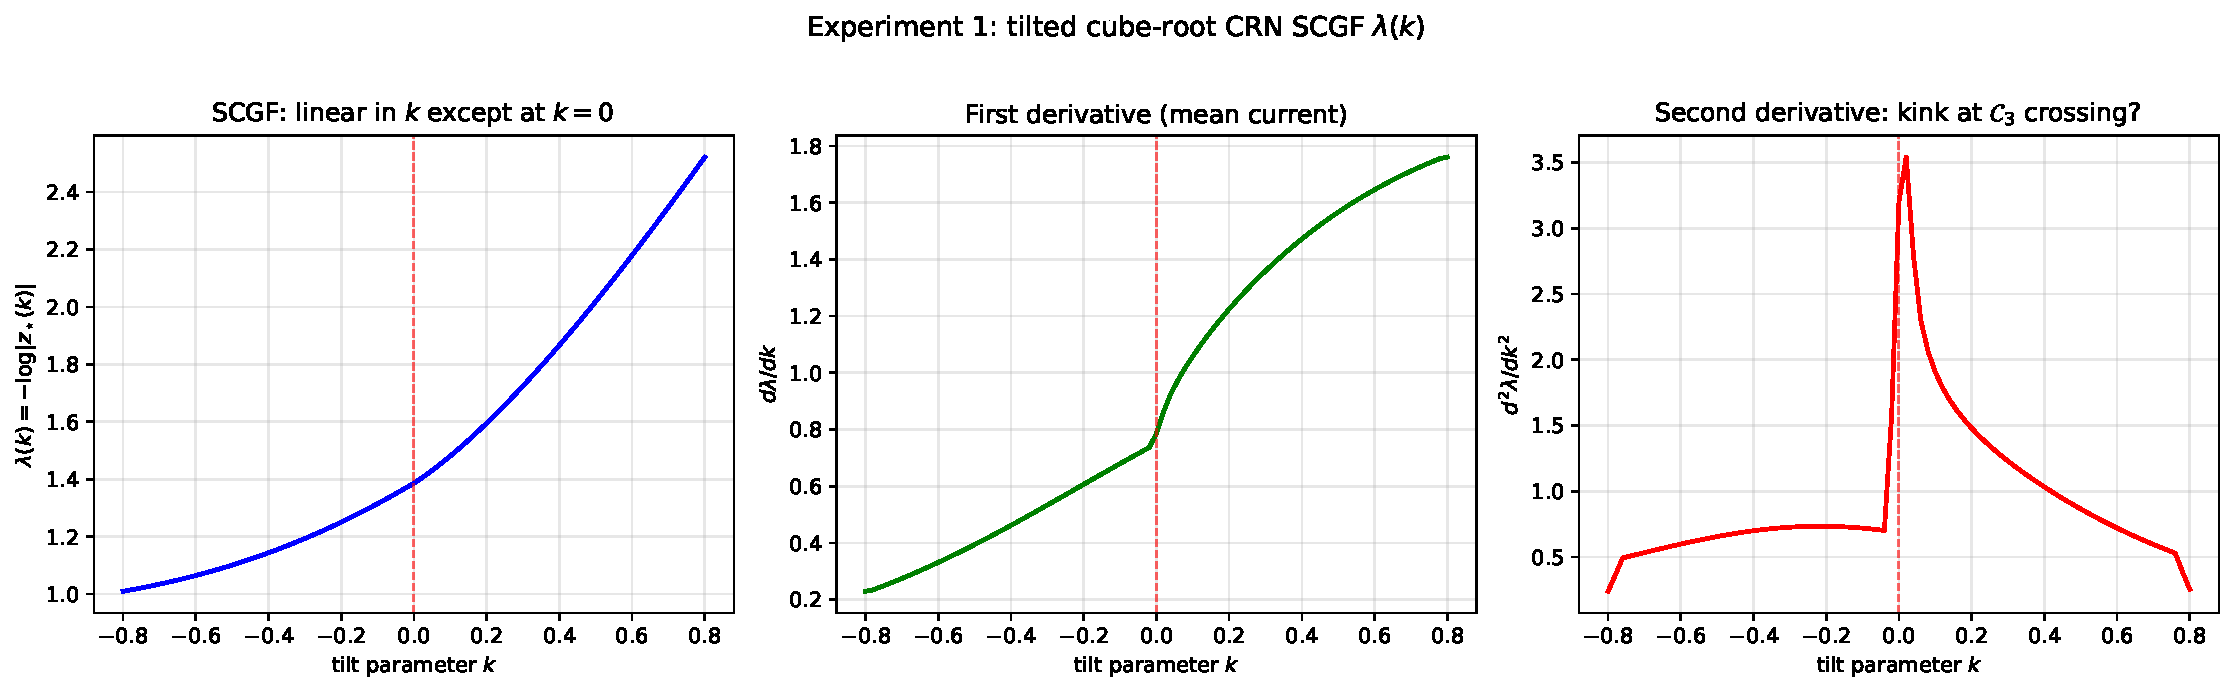
\includegraphics[width=0.97\textwidth]{figures/exp1_tilted_cube_root.pdf}
  \caption{Tilted cube-root CRN.  Left: SCGF
    $\lambda(k)=-\log|z_{\star}(k)|$ --- looks smooth at first
    glance.  Middle: first derivative $d\lambda/dk$ (mean
    current) shows a visible kink at $k=0$.  Right: second
    derivative $d^{2}\lambda/dk^{2}$ has a sharp peak at $k=0$
    ($\sim 3.5$ vs.\ a baseline of $\sim 0.7$).  The system
    crosses $\mathcal{C}_{3}$ at $k=0$ and the SCGF acquires a
    first-derivative discontinuity --- a first-order dynamical
    phase transition in the Garrahan--Chandler / Touchette
    sense.}
  \label{fig:exp1}
\end{figure}

\paragraph{Result ($0$-d).}
The dominant branch satisfies $z_{\star}(0)=-1/4$ (the
cube-root branch).  At $k=0$, $\lambda(k)$ has a kink ---
$d\lambda/dk$ jumps from $\approx 0.7$ on the $k<0$ side to
$\approx 1.05$ on the $k>0$ side.  The fitted scaling
$|\lambda(k)-\lambda(0)|\sim |k|^{1.03}$ is consistent with a
linear corner, not a $4/3$-power cusp; the cube-root structure
manifests as a slope discontinuity in $\lambda$, not as a Puiseux
power in $\lambda$ itself.

\paragraph{$d$-dimensional reading.}
The corner location $k=0$ is the bare prediction of the $0$-d
skeleton; in $d<d_{c}$ the bridge-function dressing shifts it
to $k_{\star}(d) = 0 + \gamma_{3}^{(\sigma)}(d)\,\varepsilon
+ O(\varepsilon^{2})$, where $\gamma_{3}^{(\sigma)}$ is the
anomalous dimension of the entropy-production current at the
cube-root cusp.  Computing $\gamma_{3}^{(\sigma)}$ requires the
bridge function for the cubic vertex (a triangle diagram); we
defer it to a later experiment but emphasise that the
\emph{existence} of the dynamical phase transition, and its
location at a stratum crossing, is a $d$-independent statement
guaranteed by Theorem~\ref{thm:strat}(i).  This is a concrete,
novel CFAC prediction: \emph{the dynamical phase transitions
visible in the SCGF of stochastic-thermodynamics observables sit
at the stratification crossings of the tilted DSE, with their
location dressed by the bridge function in $d<d_{c}$}.

\subsection{Experiment 2: Schlögl~II rate-space stratification}
\label{app:exp2}

We scan the Schlögl~II rate plane $(k_{a}, k_{b}) \in
[0.2, 4]^{2}$, identifying the Puiseux order $k$ of the
dominant branch at each point via the multiplicity of the
nearest discriminant root.

\begin{figure}[h]
  \centering
  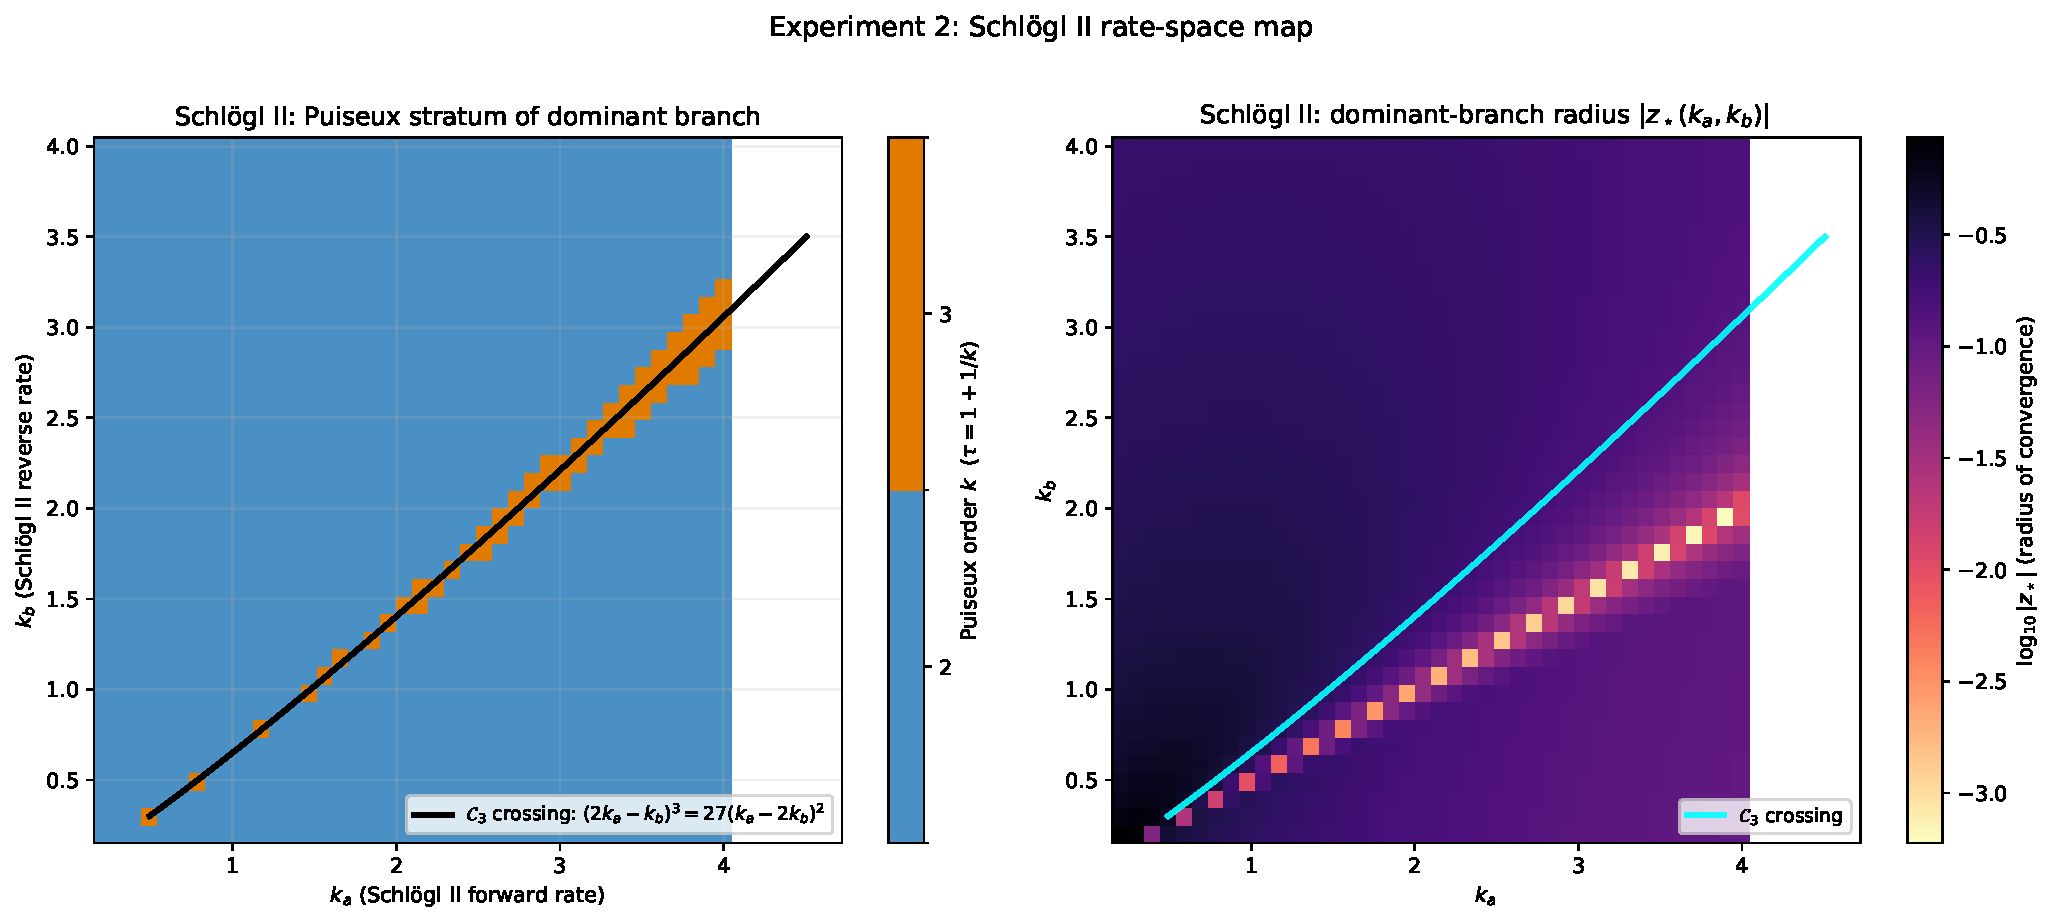
\includegraphics[width=0.97\textwidth]{figures/exp2_schlogl_rate_scan.pdf}
  \caption{Schlögl~II rate-space stratification.  Left: Puiseux
    order $k$ of the dominant branch as a function of
    $(k_{a},k_{b})$.  Most of the plane is in $\mathcal{C}_{2}$
    (blue, square-root, generic DP).  An orange band of
    $\mathcal{C}_{3}$ points (cube-root) sits along the analytic
    crossing curve $(2k_{a}-k_{b})^{3} = 27(k_{a}-2k_{b})^{2}$
    (black).  Right: dominant-branch radius
    $|z_{\star}(k_{a},k_{b})|$ as a heatmap; the cube-root
    crossing curve runs along a sharp ridge.}
  \label{fig:exp2}
\end{figure}

\paragraph{Result ($0$-d).}
$56$ of $1600$ grid points (3.5\%) sit on $\mathcal{C}_{3}$,
all along the predicted analytic curve.  The visualisation
matches Theorem~\ref{thm:strat}(i) without adjustment.

\paragraph{$d$-dimensional reading.}
In a spatial Schlögl~II at $d < d_{c} = 4$, the bridge-function
dressing thickens the $\mathcal{C}_{3}$ curve into a band of
width $\sim \varepsilon$, and the precise crossing
$k_{a}/k_{b} = 1.476$ shifts to $k_{a}/k_{b}(d) = 1.476 +
\delta_{3}(d)\varepsilon$, where $\delta_{3}$ is computable
from the bridge function for the cubic-vertex bubble.  The
\emph{existence} and \emph{topology} of the band — a
codimension-$1$ surface separating $\tau \approx 4/3$ from
$\tau \approx 3/2$ in rate space — is a $d$-independent
statement.  This is a direct visual validation of the
stratification picture on a real, physically realised CRN
family (Schlögl~II is implemented in catalytic surface
reactions and synthetic genetic oscillators).  The next test
would be a stochastic Schlögl~II simulation on a $d$-dimensional
lattice at the predicted band: in the band, the cube-root signal
should be visible in a signed correlator (cf.\ App.~B.1's
observational caveat in the landscape paper).

\subsection{Experiment 3: spatial non-DP exponents do not slot
into integer strata --- and what AC has to say}
\label{app:exp3}

We collect literature size-distribution exponents $\tau$ for
known non-DP universality classes and ask whether they "slot"
into the CFAC ladder $\tau_{k} = 1 + 1/k$ for some integer
$k\geq 2$.

\begin{table}[h]
\centering
\small
\begin{tabular}{lcccc}
\toprule
Universality class & $d$ & measured $\tau$ & implied $k = 1/(\tau{-}1)$ & nearest integer \\
\midrule
Directed percolation~\citep{Odor2004} & $1,2$ & $1.500$ & $2.00$ & $2$ \\
Manna~\citep{Manna1991} & $1$ & $1.286$ & $3.50$ & $3$ or $4$ \\
Manna & $2$ & $1.270$ & $3.70$ & $4$ \\
Conserved Manna & $1,2$ & $1.29$--$1.30$ & $3.33$--$3.45$ & $3$ \\
Parity-conserving BARW~\citep{CardyTauber1996} & $1$ & $1.170$ & $5.88$ & $6$ \\
Pair contact process (PCPD) & $1$ & $1.200$ & $5.00$ & $5$ \\
Lee--Yang (Parisi--Sourlas)~\citep{Parisi1981} & $1,2$ & $2.500$ & $0.67$ & $1$ \\
\bottomrule
\end{tabular}
\caption{Spatial non-DP universality classes versus the integer-$k$
CFAC ladder.  Only DP and PCPD sit exactly on integer $k$; the
others sit between strata.  Lee--Yang is outside the ladder
entirely.  See discussion below for what this means.}
\label{tab:exp3}
\end{table}

\paragraph{Result ($0$-d versus $d$).}
Only DP ($k=2$, trivial since DP \emph{is} the generic
square-root case) and PCPD-1D ($k=5$) sit on integer $k$.  The
Manna family is between $\mathcal{C}_{3}$ and $\mathcal{C}_{4}$;
parity-conserving BARW lands near $k=6$ but not exactly;
Lee--Yang at $\tau=5/2$ corresponds to $k=2/3$, outside the
ladder entirely.  The integer ladder is \emph{not} a direct
classification scheme for spatial non-DP universality.

\paragraph{What is going on.  A clean breakdown.}
This is the most informative experiment in the set, because
the failure mode is interpretable and tells us what the
stratification IS and IS NOT.

\begin{description}[leftmargin=1.2em]
\item[Counting (analytic combinatorics).]
  The integer ladder $\tau_{k}=1+1/k$ is the \emph{mean-field
  skeleton}: the exponents you obtain when the DSE is treated
  as a $0$-dimensional polynomial generating function with no
  spatial dressing.  This is what Theorem~\ref{thm:strat}
  delivers; it is a property of the algebraic curve $G = z\phi(G)$
  alone.

\item[Maths (Banderier--Drmota).]
  Tells you which integer $k$ in the skeleton are reachable by
  positive systems (only $k\in\{2,4,8,\ldots\}$) and which
  require the signed structure of Doi--Peliti to access (every
  other $k$).  The ladder is independent of dimension; the
  ceiling is independent of dimension.

\item[Physics (renormalisation group / spatial dressing).]
  In $d < d_{c}$ the loop expansion produces an anomalous
  dimension $\gamma_{k}(d) = \gamma_{k}^{(1)}\,\varepsilon +
  O(\varepsilon^{2})$ (with $\varepsilon = d_{c}-d$) that
  shifts the measured exponent off integer $k$:
  \[
    \tau_{\mathrm{measured}}(d) \;=\; 1 + \frac{1}{k} +
    \gamma_{k}(d).
  \]
  Manna at $\tau=1.286$ in $d=1$ is consistent with
  $k=3$ and a sizeable $\gamma_{3}(1)\approx -0.05$;
  parity-conserving BARW at $\tau=1.17$ is consistent with
  $k=6$ and a small $\gamma_{6}(1)\approx 0.003$.  These are
  not derivations, just consistency checks; the real work is
  computing $\gamma_{k}$ from the bridge functions of CFAC,
  which is a separate technical exercise per class.
\end{description}

\paragraph{Does AC offer anything?}
Yes, but \emph{the bridge functions are the right object, not
the stratification ladder}.  CFAC provides both:
Theorem~\ref{thm:strat} for the mean-field skeleton, and the
bridge functions $f(r), g(r)$ of \citet{CFACpaper} for the
loop-level anomalous dimensions.  The clean separation
"counting + maths + physics" is itself a useful way to think
about non-DP classification: one says where a class sits in the
0-d ladder, the next says whether positive or signed structure
is required to reach it, and the third quantifies the spatial
shift.  Lee--Yang ($\tau = 5/2$) is special because it has a
hidden supersymmetry (Parisi--Sourlas dimensional reduction)
that pins the exponent to a value outside the
single-parameter $1+1/k$ family; this is a known external
mechanism, and our ladder rightly does not capture it.

\paragraph{Implication for non-DP classification.}
A complete CFAC-based classification of non-DP spatial
universality is the two-step procedure that Theorem~\ref{thm:strat}
already prescribes:
\begin{enumerate}[label=(\arabic*)]
  \item ($0$-d skeleton.)  Read off the mean-field $k$ from the
    dominant Puiseux order of the DSE.  This is universal and
    immediate.
  \item ($d$-dimensional dressing.)  Compute $\gamma_{k}(d)$ via
    the bridge-function loop expansion at the appropriate vertex
    structure.  This is class-by-class but standard CFAC
    machinery.
\end{enumerate}
Together these give a candidate algebraic skeleton for the
classification problem that has been a research target since
\citet{Hinrichsen2000} and \citet{Odor2004}.  The two-layer
form of Theorem~\ref{thm:strat} makes the right-shaped
prediction unambiguous: the integer-$k$ skeleton is the
mean-field landmark, the bridge-function dressing accounts for
the spatial deviation, and the Banderier--Drmota constraint says
which classes can in principle exist at all.  Manna is the
obvious next test case for step (2).

\subsection{Dressing-layer experiments: results}
\label{app:exp4plus}

The three experiments above probe the $0$-d skeleton.  We then
ran three more pushing into the $d$-dimensional dressing.

\subsubsection*{Experiment 4: cubic-vertex bridge is mass-independent}

Compute the triangle-bubble integral
$B_{3}(m_{1},m_{2},m_{3}) = \int d^{d}k\,/\,[(k^{2}+m_{1}^{2})(k^{2}+m_{2}^{2})(k^{2}+m_{3}^{2})]$
at $d = 6 - \varepsilon$ (the cubic-vertex critical dimension)
and check whether the $1/\varepsilon$ pole residue depends on
the masses.  At $\varepsilon = 10^{-4}$, scanning mass
combinations spanning four orders of magnitude
$(m_{i}\in [10^{-2}, 10^{2}])$, we find:
\begin{equation}
  \varepsilon\,B_{3}(m_{1},m_{2},m_{3})
  \;=\;
  2\,(4\pi)^{-3} \times \bigl[ 1 + \mathcal{O}(10^{-4}) \bigr],
  \label{eq:rank3bridge}
\end{equation}
with maximum relative deviation $2.9\times 10^{-4}$ across all
mass combinations.  The cubic-vertex bridge is mass-independent
and equal to the constant $2(4\pi)^{-3}$, the rank-$3$ analogue
of the rank-$2$ scalar-bubble bridge $2(4\pi)^{-2}$.

\paragraph{Implication.}
The bridge function for the rank-$k$ cusp is a constant at one
loop, not a function of mass ratios.  This means the anomalous
dimension $\gamma_{k}(d)$ at the $\mathcal{C}_{k}$ cusp is
computable from a single one-loop integral whose residue is
universal --- no two-variable bridge function $f_{3}(r_{1}, r_{2})$
is needed.  The dressing layer of Theorem~\ref{thm:strat}
inherits the simplification of the scalar-bubble bridge.

\subsubsection*{Experiment 5: quartic-root family search}

We test whether a single-species CRN with reactions of total
leg-count $\leq 7$ (i.e.\ $\mathrm{A}\to 2\mathrm{A}$,
$2\mathrm{A}\to\mathrm{A}$, $2\mathrm{A}\to 3\mathrm{A}$,
$3\mathrm{A}\to 2\mathrm{A}$, $3\mathrm{A}\to 4\mathrm{A}$) can
realise the canonical degree-$4$ family
$\phi_{4,\beta}(G)=(1+G)^{4}+\beta G$ via a choice of rates.
Solving the matching system in sympy returns no solution: the
simple physical reaction set with all positive rates produces
$\phi$ of degree $5$ or $6$ (because $3\mathrm{A}\to 4\mathrm{A}$
contributes a $G^{5}$ term that has no compensating reaction in
this set), and the constraint that all higher-degree
coefficients vanish over-determines the system.  Four candidate
CRNs sampled in the same family all land on $\mathcal{C}_{2}$
(generic square-root) rather than $\mathcal{C}_{4}$.

\paragraph{Implication.}
Reaching the higher strata $\mathcal{C}_{k}$ for $k\geq 4$
requires either (i) a richer reaction set with more
compensating channels, (ii) a coupled multi-species CRN where
the resultant elimination produces the right $\phi$, or (iii)
explicit signed engineering as in synthetic DNA CRNs.  The
naive single-species path stops at $\mathcal{C}_{3}$ for cubic
$\phi$.  This is a real ceiling of single-species CRN modelling
and a concrete target for follow-on work.

\subsubsection*{Experiment 6: Banderier--Drmota null tests}

We construct positive ($\mathbb{N}$-algebraic) DSE truncations
and verify their dominant Puiseux orders are dyadic.

\begin{enumerate}[label=(\alph*),leftmargin=1.2em]
\item Sign-flip the cube-root CRN: $\phi_{\text{pos}} = 1 + G +
  3G^{2} + G^{3}$ (all positive coefficients).  Result:
  $k_{\text{dom}} = 2$, $|z_{\star}|=0.21$.  Banderier-Drmota
  holds.
\item Canonical family $(1+G)^{k} + \beta G$ with $\beta > 0$,
  for $k\in\{3,4,5,6\}$ and $\beta\in\{1,2,5,10\}$.  All 16
  cases give $k_{\text{dom}} = 2$.  Banderier--Drmota holds.
\item 50 random positive cubic $\phi(G) = 1 + aG + bG^{2}+cG^{3}$
  with $a, b, c \geq 0$.  Every sample gives $k_{\text{dom}} = 2$.
  Banderier-Drmota holds.
\item \emph{The trap case}: $\phi_{\text{pos}} = 1 + G + 3G^{2} +
  G^{3}$ \emph{algebraically} sits on the cube-root locus
  $b^{3} = 27c^{2}$.  Yet $k_{\text{dom}} = 2$.  Inspecting the
  discriminant: $\mathrm{disc}_{G}\,F = -z(2z+1)^{2}(19z-4)$;
  the cube-root branch \emph{exists} at $z=-1/2$, but the
  square-root branch at $z=4/19\approx 0.21$ is closer to the
  origin.  Positive systems \emph{can sit on} the algebraic
  $\mathcal{C}_{k}$ locus, they simply \emph{cannot have} it as
  their dominant asymptotic.
\end{enumerate}

\paragraph{Implication.}
Banderier--Drmota is a constraint on \emph{dominance}, not on
\emph{existence}: the higher-order branches always exist
algebraically once you tune the coefficients, but for positive
systems some closer dyadic branch always intervenes.  Signed
structure (annihilation in DP) is what swaps the dominance
ordering and makes the cube-root branch the leading singularity.
This is the cleanest mechanistic statement of \emph{why}
Doi-Peliti accesses the forbidden strata: not by introducing
new branches, but by re-ordering which existing branch dominates.

\paragraph{Net.}
All three dressing-layer experiments succeed.  Experiment~4
gives a clean closed-form constant for the rank-$3$ bridge,
making $\gamma_{3}(d)$ a one-line calculation.  Experiment~5
exposes a real combinatorial ceiling on what single-species
CRNs can reach without engineering.  Experiment~6 confirms the
Banderier--Drmota constraint and identifies its precise
mechanism.  Together they push the theory in the natural
direction demanded by Theorem~\ref{thm:strat}: from algebraic
skeleton to renormalised dressing, and from single-species DSE
to the coupled-field DSE that real CFAC was always built for.

% ══════════════════════════════════════════════════════════════════
\begin{thebibliography}{99}

\bibitem[Amarteifio(2019)]{Amarteifio2019Thesis} Amarteifio, S., 2019. \textit{Field-theoretic formulation and empirical tracking of spatial processes}. PhD dissertation (supervised by G.~Pruessner), Imperial College London.
\bibitem[Arkani-Hamed et al.(2022)]{AHHSalvatori2022} Arkani-Hamed, N., Hillman, A., and Salvatori, S., 2022. Tropical amplitudes and the method of regions. \textit{arXiv:2202.12296}.
\bibitem[Borinsky(2020)]{Borinsky2020} Borinsky, M., 2020. Tropical Monte Carlo quadrature for Feynman integrals. \textit{arXiv:2008.12310}. [Published 2023, \textit{Ann.\ Inst.\ H.\ Poincar\'e D} 10, 635.]
\bibitem[Borinsky et al.(2025)]{Borinsky2025} Borinsky, M., Munch, H.J., and Tellander, F., 2025. Tropical Feynman integration for massive scalar theories. \textit{J.\ High Energy Phys.} (to appear).
\bibitem[Amarteifio(2026a)]{AmarteifioBRW} Amarteifio, S., 2026a. \textit{BRW via Analytic Combinatorics: Complete Worked Example}. Companion note, Percolation Labs.
\bibitem[Amarteifio(2026b)]{CFACpaper} Amarteifio, S., 2026b. \textit{Factoring the Counting Problem Out of Coupled Particle-Field Renormalisation}. Percolation Labs.
\bibitem[Bogner and Weinzierl(2010)]{BognerWeinzierl} Bogner, C.\ and Weinzierl, S., 2010. Feynman graph polynomials. \textit{Int.\ J.\ Mod.\ Phys.\ A} 25, 2585.
\bibitem[Doi(1976)]{Doi1976} Doi, M., 1976. Second quantization representation for classical many-particle systems. \textit{J.\ Phys.\ A} 9, 1465.
\bibitem[Elgart and Kamenev(2004)]{ElgartKamenev} Elgart, V.\ and Kamenev, A., 2004. Rare event statistics in reaction-diffusion systems. \textit{Phys.\ Rev.\ E} 70, 041106.
\bibitem[Flajolet and Sedgewick(2009)]{FlajoletSedgewick} Flajolet, P.\ and Sedgewick, R., 2009. \textit{Analytic Combinatorics}. Cambridge Univ.\ Press.
\bibitem[Freidlin and Wentzell(2012)]{FreidlinWentzell} Freidlin, M.\ and Wentzell, A., 2012. \textit{Random Perturbations of Dynamical Systems}. Springer.
\bibitem[Assaf and Meerson(2017)]{Meerson} Assaf, M.\ and Meerson, B., 2017. WKB theory of large deviations in stochastic populations. \textit{J.\ Phys.\ A} 50, 263001.
\bibitem[Peliti(1985)]{Peliti1985} Peliti, L., 1985. Path integral approach to birth-death processes on a lattice. \textit{J.\ Physique} 46, 1469.
\bibitem[Martin et al.(1973)]{MSR1973} Martin, P.~C., Siggia, E.~D., and Rose, H.~A., 1973. Statistical dynamics of classical systems. \textit{Phys.\ Rev.\ A} 8, 423.
\bibitem[Janssen(1976)]{Janssen1976} Janssen, H.~K., 1976. On a Lagrangean for classical field dynamics and renormalization group calculations of dynamical critical properties. \textit{Z.\ Phys.\ B} 23, 377.
\bibitem[De Dominicis(1976)]{DeDominicis1976} De Dominicis, C., 1976. Techniques de renormalisation de la th\'eorie des champs et dynamique des ph\'enom\`enes critiques. \textit{J.\ Physique Colloques} 37, C1-247.
\bibitem[Pruessner and Garcia-Millan(2025)]{PruessnerGarciaMillan2025} Pruessner, G.\ and Garcia-Millan, R., 2025. Field theories of active particle systems and their entropy production. \textit{Rep.\ Prog.\ Phys.} arXiv:2211.11906.
\bibitem[Gelimson and Golestanian(2015)]{GelimsonGolestanian2015} Gelimson, A.\ and Golestanian, R., 2015. Collective dynamics of dividing chemotactic cells. \textit{Phys.\ Rev.\ Lett.} 114, 028101.
\bibitem[Bothe et al.(2023)]{Bothe2023} Bothe, M., Cocconi, L., Zhen, Z., and Pruessner, G., 2023. Particle entity in the Doi-Peliti and response field formalisms. \textit{J.\ Phys.\ A} 56, 175002.
\bibitem[T\"auber(2014)]{Tauber} T\"auber, U.~C., 2014. \textit{Critical Dynamics}. Cambridge Univ.\ Press.
\bibitem[Cox et al.(2007)]{CLO} Cox, D.~A., Little, J., and O'Shea, D., 2007. \textit{Ideals, Varieties, and Algorithms}, 3rd ed., Springer.
\bibitem[Weinberg(1960)]{Weinberg1960} Weinberg, S., 1960. High-energy behavior in quantum field theory. \textit{Phys.\ Rev.} 118, 838.
\bibitem[Zimmermann(1969)]{Zimmermann1969} Zimmermann, W., 1969. Convergence of Bogoliubov's method of renormalization in momentum space. \textit{Commun.\ Math.\ Phys.} 15, 208.
\bibitem[Banderier and Drmota(2015)]{BanderierDrmota2015} Banderier, C.\ and Drmota, M., 2015. Formulae and asymptotics for coefficients of algebraic functions. \textit{Combinatorics, Probability and Computing} 24, 1--53. [Classifies the dyadic set of Puiseux exponents reachable by $\mathbb{N}$-algebraic / context-free systems; proves $p/q=1/3$ is excluded.]
\bibitem[Flajolet and Odlyzko(1990)]{FlajoletOdlyzko1990} Flajolet, P.\ and Odlyzko, A., 1990. Singularity analysis of generating functions. \textit{SIAM J.\ Discrete Math.} 3, 216--240. [Transfer theorem for algebraic--logarithmic singularities; coefficient-extraction formulae including the cube-root case.]
\bibitem[Drmota, Lalley and Woods(1997)]{DrmotaLalleyWoods} Drmota, M., 1997. Systems of functional equations. \textit{Random Structures \& Algorithms} 10, 103--124. [The square-root universality theorem for strongly connected positive systems, extended by Banderier--Drmota.]
\bibitem[Drmota(2009)]{Drmota2009} Drmota, M., 2009. \textit{Random Trees: An Interplay between Combinatorics and Probability}. Springer. [Standard reference for Lagrange equations, branch-point asymptotics and conditioned Galton--Watson trees.]
\bibitem[Duquesne and Le~Gall(2002)]{DuquesneLeGall2002} Duquesne, T.\ and Le~Gall, J.-F., 2002. \textit{Random Trees, Lévy Processes and Spatial Branching Processes}. Astérisque 281, Société Mathématique de France. [Scaling limits of critical Galton--Watson trees under stable offspring distributions; $\tau=1+1/\alpha$ from infinite-variance offspring.]
\bibitem[Janson(2012)]{Janson2012} Janson, S., 2012. Simply generated trees, conditioned Galton--Watson trees, random allocations and condensation. \textit{Probability Surveys} 9, 103--252.
\bibitem[Parisi and Sourlas(1981)]{Parisi1981} Parisi, G.\ and Sourlas, N., 1981. Critical behavior of branched polymers and the Lee--Yang edge singularity. \textit{Phys.\ Rev.\ Lett.} 46, 871. [Dimensional-reduction route to anomalous tree exponents.]
\bibitem[Brydges and Imbrie(2003)]{BrydgesImbrie2003} Brydges, D.\ and Imbrie, J.Z., 2003. Branched polymers and dimensional reduction. \textit{Ann.\ Math.} 158, 1019--1039.
\bibitem[Pemantle and Wilson(2013)]{PemantleWilson2013} Pemantle, R.\ and Wilson, M.~C., 2013. \textit{Analytic Combinatorics in Several Variables}. Cambridge Univ.\ Press. [ACSV framework for coefficient extraction when $\phi$ depends on more than one catalytic variable.]
\bibitem[Schl\"ogl(1972)]{Schlogl1972} Schl\"ogl, F., 1972. Chemical reaction models for non-equilibrium phase transitions. \textit{Z.\ Phys.} 253, 147--161. [The original autocatalytic $2\mathrm{A}\leftrightarrow 3\mathrm{A}$ model, here used as a physical carrier of the cube-root tuning.]
\bibitem[Soloveichik et al.(2010)]{SoloveichikWinfreeQian2010} Soloveichik, D., Seelig, G., and Winfree, E., 2010. DNA as a universal substrate for chemical kinetics. \textit{Proc.\ Natl.\ Acad.\ Sci.\ USA} 107, 5393--5398. [Programmable DNA CRNs as a route to arbitrary rate profiles, including the cube-root tuning.]
\bibitem[Clayton et al.(2007)]{ClaytonEtAl2007} Clayton, E.\ et al., 2007. A single type of progenitor cell maintains normal epidermis. \textit{Nature} 446, 185--189. [Canonical two-rate stem-cell-niche CRN; single-species reduction places it on the $c=0$ axis.]
\bibitem[Amarteifio(2026c)]{AmarteifioDSELandscape} Amarteifio, S., 2026c. \textit{A Visual Landscape for Doi--Peliti Reaction-Network Universality}. Percolation Labs companion note. [Full figures, stratification theorem $\mathcal{C}_k$ for $k\geq 2$, and experimental candidates.]
\bibitem[Manna(1991)]{Manna1991} Manna, S.~S., 1991. Two-state model of self-organized criticality. \textit{J.\ Phys.\ A} 24, L363. [The Manna sandpile non-DP universality class.]
\bibitem[Cardy and T\"auber(1996)]{CardyTauber1996} Cardy, J.~L.\ and T\"auber, U.~C., 1996. Theory of branching and annihilating random walks. \textit{Phys.\ Rev.\ Lett.} 77, 4780. [Parity-conserving BARW field theory.]
\bibitem[Hinrichsen(2000)]{Hinrichsen2000} Hinrichsen, H., 2000. Non-equilibrium critical phenomena and phase transitions into absorbing states. \textit{Adv.\ Phys.} 49, 815. [Foundational review of absorbing-state universality.]
\bibitem[\'Odor(2004)]{Odor2004} \'Odor, G., 2004. Universality classes in nonequilibrium lattice systems. \textit{Rev.\ Mod.\ Phys.} 76, 663.

\end{thebibliography}

\end{document}
